\chapter{Implementation}
\section{Introduction}
Simulations have been done in MATLAB.
\section{Particle Swarm Optimization}
The PSO\footnote{PSO stands for Particle Swarm Optimization.} algorithm was first introduced in 1995 
\cite{PSO_original}, and it has since proven to be a powerful tool for solving various optimization problems. 
In the standard PSO algorithm, a population of particles is randomly initialized to represent potential candidate 
solutions for the optimization problem. Each particle relies on two important pieces of information: its individual 
best, referred to as \textit{pbest}, and the global best across the entire population, referred to as \textit{gbest}. 
These two values guide the search direction of all particles over the search space. The evaluation of the 
\textit{pbest} for each particle and the \textit{gbest} for the entire population is determined by the function 
that needs to be optimized.

\par In our implementation, each particle corresponds to an individual drone 
within the swarm, and the velocity and position of each drone are updated in 
accordance with the aforementioned standard PSO algorithm. Let $\mathbf{p}_i \in \mathbb{R}^2$ 
for $i = 1, 2, \dots, n$ represent the position vectors of the drones in the 2D plane, 
where $n$ is the total number of drones. The motion of each particle is governed 
by two fundamental equations: the velocity update equation (Eq.~\ref{eq:velocity}) and 
the position update equation (Eq.~\ref{eq:position}).
\begin{align}
    \mathbf{v}_{i}(t+1) &= \omega \, \mathbf{v}_{i}(t) + c_1 r_1 \left( \mathbf{pbest}_{i}(t) - \mathbf{p}_{i}(t) \right) 
    + c_2 r_2 \left( \mathbf{gbest}(t) - \mathbf{p}_{i}(t) \right) \label{eq:velocity} \\
    \mathbf{p}_{i}(t+1) &= \mathbf{p}_{i}(t) + \mathbf{v}_{i}(t+1) \label{eq:position}
\end{align}
    
where $\mathbf{p}_i$, $\mathbf{pbest}_i$, and $\mathbf{gbest}$ represent the position vector of the $i$-th particle, 
the $i$-th particle's individual best position vector, and the global best position vector, 
$\omega$ is the inertia weight, $c_1$ and $c_2$ are positive constants, and
$r_1$ and $r_2$ are random variables uniformly distributed over the interval $[0, 1]$.

\par In the standard PSO algorithm, there is only one global best particle, 
which means that only one optimal solution can be found. This limitation 
poses a challenge when dealing with our problem, where we are looking for multiple sources, 
and therefore, multiple local and global optima exist. To address this challenge, 
we employ the same strategy of a modified version of the PSO algorithm \cite{PSO_IMPORTANT}. 
In this modification, the swarm is divided into $M$ subpopulations, each tasked with exploring 
different regions of the search space. Following this idea, the \textit{gbest} is referred to as 
the best particle of each subpopulation, not as the global best particle in the whole population. 
This means that these $M$ best particles are separately able to catch different optima, at most $M$ optima.

\par The function \texttt{sort\_drones\_in\_groups} returns the number of groups and sorts the 
particles in different groups based on the following logic (see Algorithm~\ref{alg:sort_drones_in_groups}):
\begin{algorithm}[H]
    \caption{\texttt{sort\_drones\_in\_groups} (MATLAB function)}\label{alg:sort_drones_in_groups}
    \begin{algorithmic}[1]
    \State \textbf{Inputs:}
    \State $n\_drones$: Number of drones available for assignment
    \State $n\_sources$: Number of sources to which drones need to be assigned
    \State \textbf{Outputs:}
    \State $group\_indices$: A vector of size $n\_drones$ indicating the assigned group
    \State $n\_groups$: The obtained number of groups
    \If{$n\_particles > n\_sources$}
        \State Assign at least one particle to each group, following mathematical order
        \State Randomly assign remaining particles to existing groups
    \ElsIf{$n\_particles = n\_sources$}
        \State Assign each particle to a unique group
    \Else
        \State Orderly assign particles up to $n\_drones$
    \EndIf
    \State Set the number of groups: $n\_groups = max(group\_indices)$
    \end{algorithmic}
\end{algorithm}

\par Note that the function \texttt{sort\_drones\_in\_groups} ensures the creation of sufficient groups 
for the localization of multiple sources only when the number of drones is equal to or greater than 
the number of sources.

\subsection{Exploration phase}
\par Unlike the modified PSO algorithm, in our implementation, the drones are not randomly initialized. 
At the start of the simulation, all drones are located at the origin of the search space. 
An Exploration Phase begins where the PSO algorithm is not yet employed. 
During this phase, the drones move according to predefined trajectories at maximum speed $v_{\text{max}}$. 
The trajectories are determined based on the number of drones and follow a radial pattern, as shown in Figure \ref{fig:exploration_pattern}. 
The drones follow these trajectories until they have covered a distance $travel\_distance$ equivalent to half the boundary of the search space.
The goal each drone needs to reach is computed using the following Algorithm~\ref{alg:exploration_goals}:

\begin{algorithm}[H]
    \caption{\texttt{exploration\_goals} (MATLAB function)} \label{alg:exploration_goals}
    \begin{algorithmic}[1]
        \State \textbf{Input:} $n\_{drones}$, $x\_{max}$
        \State \textbf{Output:} $goals$ 
        \State Initialize an empty array $goals$
        \State Set $angle\_step = 360 / n\_{drones}$
        \State Set $travel\_distance = x\_{max} / 2$ 
        \For{each drone $i = 1, 2, \dots, n\_{drones}$}
            \State Get angle for the current drone: $drone\_angle = i \cdot angle\_step$
            \State Calculate slope: $m = \tan(\texttt{deg2rad}(drone\_angle))$
            \If{$drone\_angle > 315$ \textbf{or} $drone\_angle \leq 45$} 
                \State $goal = [travel\_distance, m \cdot travel\_distance]$ \Comment{1st quadrants}
            \ElsIf{$drone\_angle > 45$ \textbf{and} $drone\_angle \leq 135$}
                \State $goal = [travel\_distance / m, travel\_distance]$ \Comment{2nd quadrant}
            \ElsIf{$drone\_angle > 135$ \textbf{and} $drone\_angle \leq 225$}
                \State $goal = [-travel\_distance, m \cdot -travel\_distance]$ \Comment{3rd quadrant}
            \ElsIf{$drone\_angle > 225$ \textbf{and} $drone\_angle \leq 315$}
                \State $goal = [-travel\_distance / m, -travel\_distance]$ \Comment{4th quadrant}
            \EndIf
            \State Store the goal for drone $i$ in $goals[i]$
        \EndFor
        \State Return $goals$
    \end{algorithmic}
\end{algorithm}

where $angle\_step$ is the angular increment to uniformly divide the space, $drone\_angle$ represents the angle assigned to each drone, determining its trajectory, 
while $m$ is the slope of the trajectory calculated from the drone's angle. 

\begin{figure}
    \centering
    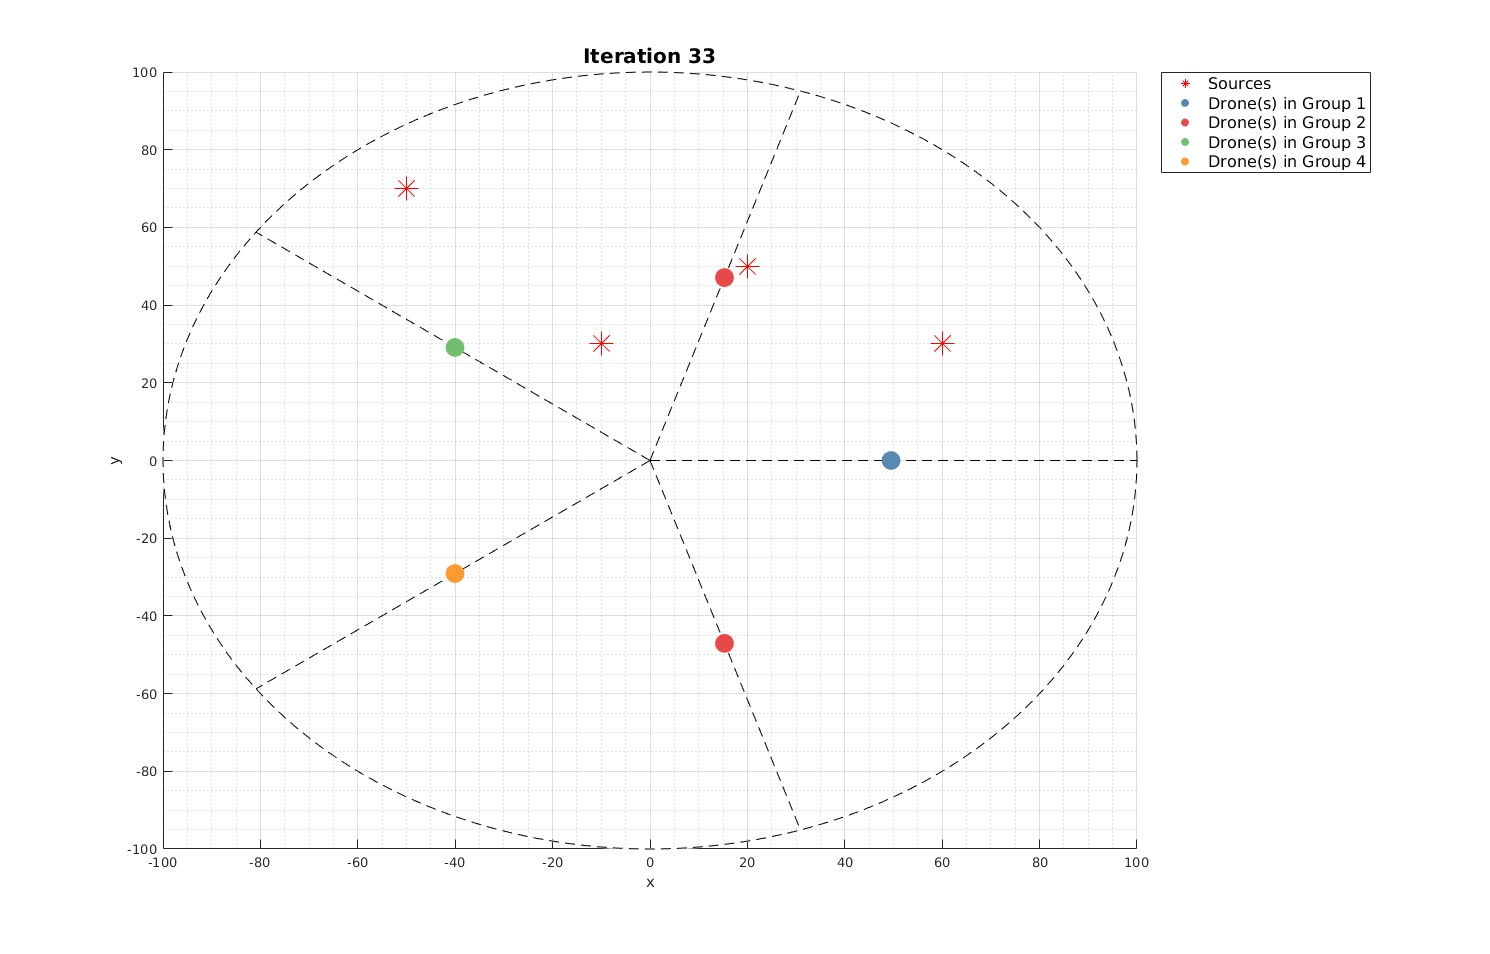
\includegraphics[width=\textwidth]{images/exploration_pattern.jpg} 
    \caption{Radial exploration pattern for 5 drones at the end of the Exploration Phase.}
    \label{fig:exploration_pattern}
\end{figure}

\section{Exploitation Phase}
\section{Velocity Update}
At each time step, the velocity update of the standard PSO algorithm is modified in order to favor the complete 
exploration of the search space and to avoid premature convergence to local maxima, where a source is not present. 
A uniform random noise is added to the velocity of each particle to achieve a \textit{persistence of excitation},
allowing every drone to explore new and different directions, 
as described in the following formula:
\[
\mathbf{v}_i = \mathbf{v}_i + \beta \cdot \mathbf{r} \cdot ||\mathbf{v}_i||
\]
where:
\begin{itemize}
    \item \(\beta\) is an hyperparameter chosen in the [0,1] range.
    \item \(\mathbf{r} \sim \mathcal{U}(-1, 1)\) represents a random vector where each component is uniformly distributed between \(-1\) and \(1\).
    \item \(||\mathbf{v}_i||\) is the magnitude of the velocity vector of particle \(i\).
\end{itemize}
Furthermore, not only because of the physical velocity limitations of the drones, but also to ensure smoother updates 
and prevent instability due to excessive velocity, we clamp the velocity of each drone 
to a maximum value \(v_{\text{max}}\):
\[
\mathbf{v}_i = 
\begin{cases} 
\mathbf{v}_{\text{max}}, & \text{if } ||\mathbf{v}_i|| \geq v_{\text{max}} \\
\mathbf{v}_i, & \text{otherwise}
\end{cases}
\]

\subsection{Exlusion Zones Mechanism}

\subsection{Complete Modified PSO}
\begin{algorithm}
    \caption{Particle Swarm Optimization for Multi-Source Localization}\label{alg:PSO}
    \begin{algorithmic}[1]
        \State Initialize group best positions $G_{\text{best}}$ and values $V_{\text{best}}$
        \State Assign each drone to a group corresponding to one of the sources
        
        \For{each iteration $t = 1$ to $n\_iterations$}
            \For{each drone $i$}
                \State Update velocity:
                \[
                    v_i(t+1) = \omega v_i(t) + c_1 \cdot r_1 \cdot (p_{\text{best}} - p_i(t)) + c_2 \cdot r_2 \cdot (G_{\text{best}} - p_i(t))
                \]
                \State Limit the velocity to $v_{\text{max}}$
                \State Update position:
                \[
                    p_i(t+1) = p_i(t) + v_i(t+1)
                \]
                \State Apply boundary conditions to keep $p_i(t+1)$ within $bounds$
                
                \For{each other drone $j \neq i$}
                    \If{$||p_i(t+1) - p_j(t+1)|| \leq r_{\text{comm}}$}
                        \If{drone $i$ or $j$ has found a source}
                            \State Share exclusion zones between drones
                        \EndIf
                    \EndIf
                \EndFor
                
                \State Check if drone $i$ is within an exclusion zone
                \If{drone $i$ is in an exclusion zone}
                    \If{drone $i$ is not alone in its group}
                        \State Reassign drone $i$ to a new group
                    \Else
                        \State Move drone $i$ away from the exclusion zone
                        \State Introduce randomness to position and reset personal best $p_{\text{best}}$
                    \EndIf
                \Else
                    \State Evaluate NSS at $p_i(t+1)$
                    \If{current NSS $>$ personal best NSS}
                        \State Update personal best $p_{\text{best}}$
                    \EndIf
                    \If{current NSS $>$ group best NSS}
                        \State Update group best $G_{\text{best}}$
                    \EndIf
                \EndIf
            \EndFor
        \EndFor
        
        \State Return estimated source positions
    \end{algorithmic}
\end{algorithm}

    